\chapter{联邦学习的自适应加噪机制}
\label{ch3}

最近研究表明深度神经网络容易受到对抗样本的攻击。为了解决这个问题,一些工作通过向图像中添加高斯噪声来训练网络,从而提高网络防御对抗样本的能力,但是该方法在添加噪声时并没有考虑到神经网络对图像中不同区域的敏感性是不同的。针对这一问题,提出了梯度指导噪声添加的对抗训练算法。该算法在训练网络时,根据图像中不同区域的敏感性向其添加自适应的噪声,在敏感性较大的区域上添加较大的噪声,抑制网络对图像变化的敏感程度,在敏感性较小的区域上添加较小的噪声,提高其分类精度。
提出一种基于数据差分隐私保护的随机梯度下降算法。引入范数剪切与附加高斯噪声操作,对传统梯度更新策略进行改进。为衡量每次迭代过程中对数据隐私性的破坏,提出隐私损失累积函数在迭代过程中对数据隐私性的侵犯程度进行度量。

\section{模型设计}

\subsection{模型概览}
如图一所示,在我们的系统模型中,有两方,即云服务器和用户。

\textbf{云服务器}:云服务器事先与用户协商一个网络框架。然后,服务器通过公共数据训练一个初始模型,然后将初始模型的参数广播给用户。用户在本地训练各自的模型后,云服务器收集用户发送的模型梯度,并更新全球模型。

\textbf{用户}:用户下载由云服务器初始化的模型参数。然后,每个用户在本地数据集上训练私人模型。最后,用户将本地模型的扰动梯度发送到云服务器。

\subsection{威胁模型}
我们认为云服务器是一个 "诚实但好奇 "的实体。也就是说,服务器将遵循与所有用户的协议。然而,通过利用完全访问用户梯度的便利,它也试图在训练过程中获得额外的信息。出于这个原因,我们的ANFL的目标是保护发送到服务器的本地梯度不被推断出任何关于用户的额外信息。


\subsection{联邦学习中的差分隐私}

所谓在联邦学习中使用差分隐私,主要流程如下所示:
- 本地计算
客户端 $\mathrm{i}$ 根据本地数据库 $\mathcal{D}_{\mathrm{i}}$ 和接受的服务器的全局模型 $\mathrm{w}_{\mathrm{G}}^{\mathrm{t}}$ 作为本地的参数,即 $\mathrm{w}_{\mathrm{i}}^{\mathrm{t}}=\mathrm{w}_{\mathrm{G}}^{\mathrm{t}}$, 进 行梯度下降策略进行本地模型训练得到 $\mathrm{w}_{\mathrm{i}}^{\mathrm{t}+1} \quad(\mathrm{t}$ 表示当前round) 。
- 模型扰动
每个客户端产生一个随机噪音 $\mathrm{n}, \mathrm{n}$ 是符合高斯分布的,使用 $\overline{\mathbf{w}_{\mathrm{i}}}^{\mathrm{t}+1}=\mathrm{w}_{\mathrm{i}}^{\mathrm{t}+1}+\mathrm{n}$ 扰动本地模型 (这里注意w是一个矩阵,那么n就对矩阵的每一个元素产生噪音)。
- 模型聚合
服务器使用FedAVG算法聚合从客户端收到的 $\overline{\mathrm{w}}_{\mathrm{i}} \mathrm{t}+1$ 得到新的全局模型参数 $\mathrm{w}_{\mathrm{G}}^{\mathrm{t}+1}$, 也就是扰动过的 模型参数。
- 模型广播
服务器将新的模型参数广播给每个客户端。
- 本地模型更新
每个客户端接受新的模型参数,重新进行本地计算。
以上是利用差分隐私进行联邦学习梯度参数隐私保护的典型过程。当然也有一些变体, 但是大体上都是这个思路。


我们用层间相关性传播(LRP)算法将输出分解到每一层。关于LRP算法的更多细节,我们将在以下部分进行介绍。每个用户都在本地对原始数据进行训练前馈操作,这可以获得一个新的数据操作,从而获得本地模型的输出。根据相邻层之间的线性关系,在$k-t h$ 层的神经元的贡献$C_{a_{i}}^{l_{k}}\left(x_{i}\right)$等于连接到神经元$a_{i}$的相邻层的贡献之和:

$$
C_{a_{i}}^{l_{k}}\left(x_{i}\right)=\sum_{a_{j} \in l_{k+1}} C_{a_{i} \leftarrow a_{j}}^{l_{k} \leftarrow l_{k+1}}\left(x_{i}\right)
$$


例如,如图2所示,我们有:
$$
C_{a_{7}}^{l_{2}}\left(x_{i}\right)=\sum_{a_{j} \in l_{3}} C_{a_{7} \leftarrow a_{j}}^{l_{2} \leftarrow l_{3}}\left(x_{i}\right)=C_{a_{7} \leftarrow a_{8}}^{l_{2} \leftarrow l_{3}}\left(x_{i}\right)+C_{a_{7} \leftarrow a_{9}}^{l_{2} \leftarrow l_{3}}\left(x_{i}\right)
$$

其中,"$_leftarrow$"表示两部分之间的连接关系。"$l_{2} \l_{3}$ " 是指深度神经网络(DNNs)中$2-t h$层和第3层之间相邻层的连接关系。
当$k-t h$层为输出层时,我们有:
$$
C_{a_{i}}^{l_{k}}\left(x_{i}\right)=f\left(x_{i}, \omega_{i}^{r}\right)
$$

\section{鲁棒性验证框架的整体介绍}
\begin{figure}[!hbt]
\centering
	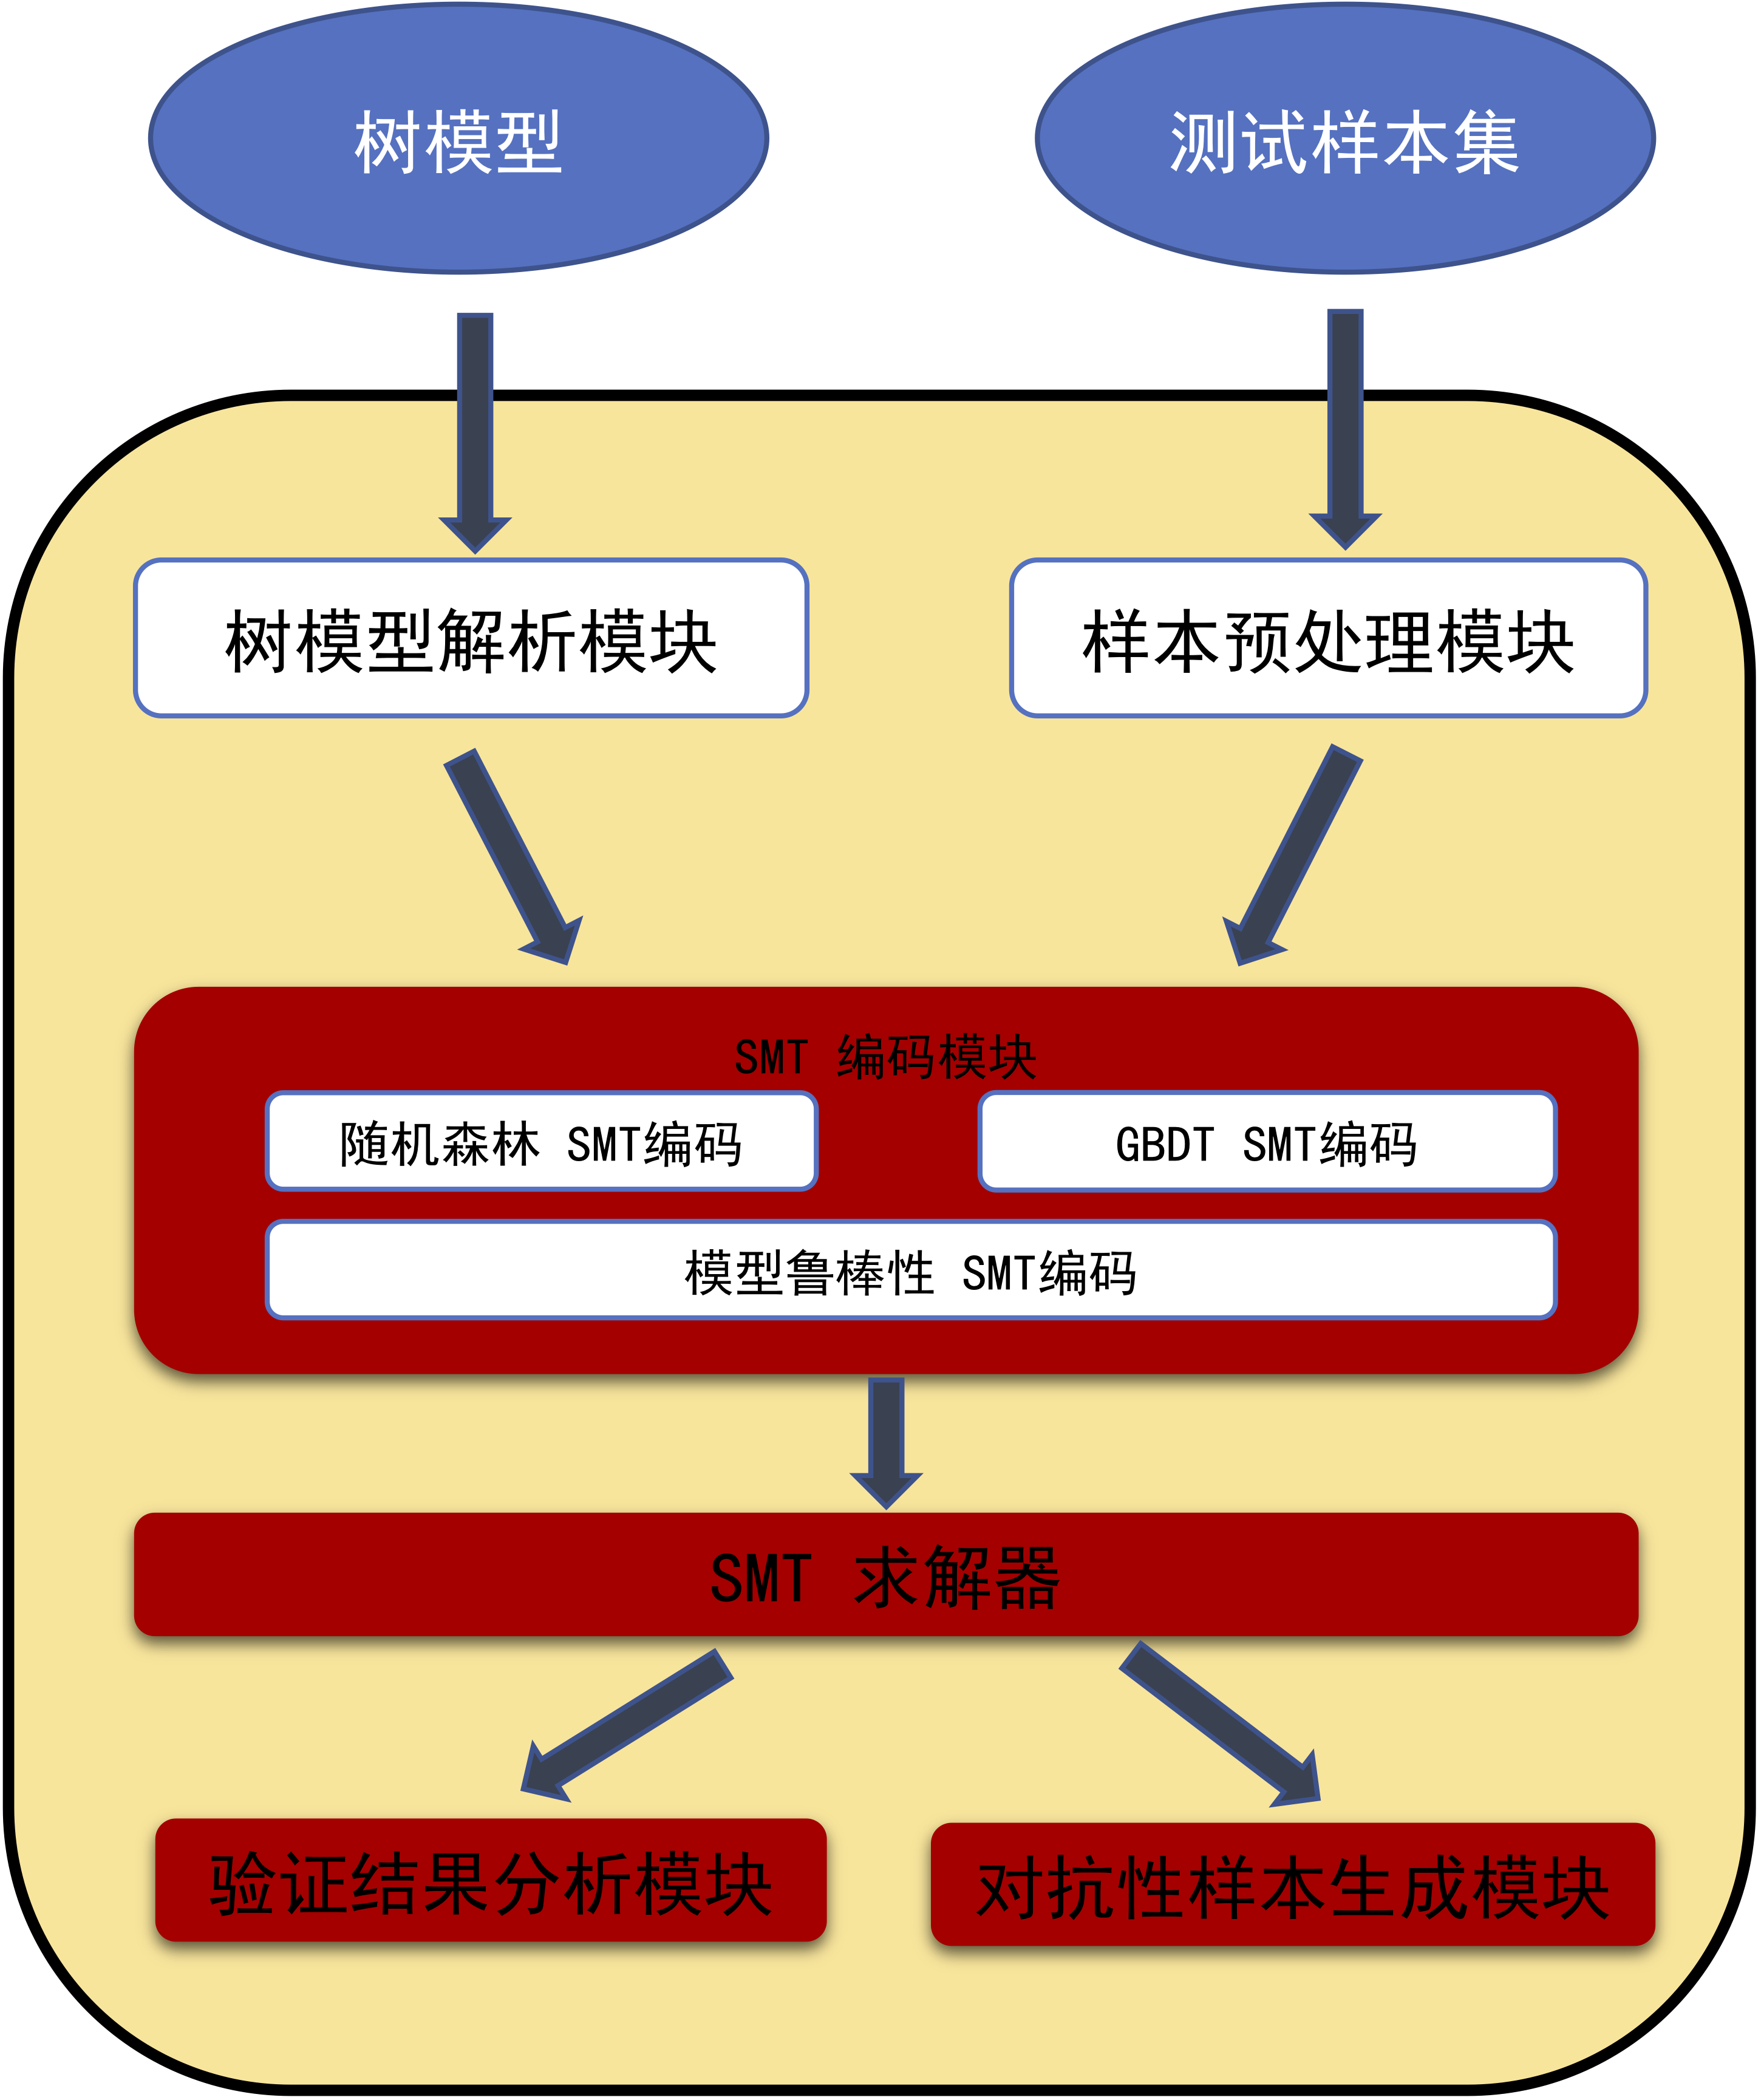
\includegraphics[scale=0.7]{fig2/C3/LBXYZKJT.png}%鲁棒性验证框架图
	\caption{验证框架图}
	\label{fig:鲁棒性验证框架图}	
\end{figure}
图\ref{fig:鲁棒性验证框架图}展示了树模型鲁棒性验证的框架图。框架的输入包括树模型的源文件和测试样本集。首先,需要对树模型进行结构解析,主要是提取树模型的结点信息。同时样本预处理模块需要对测试样本集进行数据预处理。接下来的 SMT 编码模块是我们的工作的核心。我们的验证框架需要支持树模型的两个重要实现:随机森林模型和 GBDT模型。因此,我们实现了这两种模型的编码器。SMT 编码模块主要的任务是把树模型和待验证的样本鲁棒性质编码成 SMT 公式,以便可以利用 SMT 求解器进行可满足性求解。当 SMT 求解器返回求解结果之后,验证结果分析模块会对结果进行统计分析。同时对于鲁棒性不满足的情况,在对抗性样本生成模块中会生成该样本的对抗性样本。我们将在以下小节详细介绍各个模块的内容和实现原理。

\section{树模型解析模块}
树模型解析模块主要是用于解析树模型的内部结构。我们首先需要对待验证的树模型进行结构解析,从而获取到该模型的一些内部信息为之后的 SMT 编码模块做准备。

我们知道,无论是随机森林还是 GBDT模型都是决策树的集合。所以在解析模块中,我们会对集合中所有的单棵决策树进行解析,并保存成相应的数据结构。一般来说,决策树的结构为二叉树。决策树 T 可以被定义为一个公式  $t: X^{d} \rightarrow Y^{m}$ ,对于一个输入样本向量 $x\in X^d$ 且 $x=<a_1,...,a_d>$,决策树 T 可返回一个预测结果 $y\in Y^m$。 其中 $X^d$ 表示输入样本的特征空间,特征数量为 $d$, $Y^m$表示输出空间, $m$ 表示预测类别个数。我们可以将决策树定义成一个3元组 $T = \langle N,L,V \rangle$。
\begin{define}[决策树]\label{决策树}
一颗决策树 T是一个3元组$ \langle N,L,V \rangle$, 其中:
\begin{enumerate}
	\item  $N=\{n_0,n_1,...,n_k\}$是内部结点的集合,其中 $n_0$ 表示根结点。对于每一个内部结点 $n\in N$ 都会与一个特征阈值表达式$s_n=(a_i,n_i)$相对应,如果 $s_n=a_i\le n_i$ 为 True, 则将当前结点的孩子结点左孩子结点$n_l\in N$。相反,如果 $s_n$为 False 则为右孩子结点 $n_r\in N$。
	\item  $L = \{l_0,...,l_j\}$是叶子结点的集合。
	\item $V=\{v_{l_{0}},...,v_{l_{j}}\}$ 是叶子结点的值集合, 其中$v_{l_{0}}\in V$代表的是叶子结点$l_0\in L$的叶子结点的值。如果树为分类决策树,则$v_{l}=\left\{p_{i} \mid 0 \leq i \leq m, \sum_{i=0}^{m} p_{i}=1\right\}$,其中$p_i$ 代表的是类别 $i$的预测概率,取值不能大于 1;如果树为回归决策树,则 $v_l=q_i$,其中$q_i$ 为回归值。
\end{enumerate}
\end{define}
总的来说,树模型解析模块会将树模型集合中的各个子树按照定义\ref{决策树}保存成对应的数据结构,为SMT 编码模块提供模型的结构信息。

\section{样本预处理模块}
有些情况下,我们得到的样本数据集会存在缺失,格式不统一等问题,所以在使用之前,应该进行预处理。样本预处理模块提供了一些基本的数据处理功能,如缺失值插补,去重等。我们利用 Pandas,Numpy 等第三方库实现了该模块。

\section{SMT编码模块}
为了能够使用 SMT 理论来验证树模型的鲁棒性,我们需要将树模型编码为 SMT 公式。SMT 编码模块是整个验证框架的核心模块。我们将在本节详细阐述随机森林和 GBDT 模型的SMT公式的编码过程。

\subsection{决策树的SMT编码}
在树模型解析模块,我们已经将模型集合中的决策树按照定义\ref{决策树}解析完成,在本小节我们详细描述了如何根据决策树构建其对应布尔逻辑表达式的过程,为之后整个树模型的SMT 公式的编码做准备。

首先我们从编码决策树中的一条路径开始,如果有一棵决策树$T = \langle N,L,V \rangle$,  $ l \in L$表示其叶子结点, 则叶子结点的决策路径公式$w(l)$ 如下:
\begin{equation}\label{eq:roadFormula}
\omega(l): \bigwedge_{n \in \mathrm{N}_{1}}\left(s_{n}\right) \wedge\left(o=v_{l}\right), s_{n}=\left\{\begin{array}{ll}
a_{i} \leq \eta_{i} & n_{c}=n_{l} \\
a_{i}>\eta_{i} & n_{c}=n_{r}
\end{array}\right.
\end{equation}
其中 $N_l$表示从根结点$n_0$ 到叶子结点 $l$的内部结点集合,$o$为叶子值$v_l$的约束变量,$n_c$ 表示结点$n$的一个孩子结点。$s_n$为结点$n$所对应的特征阈值条件式。如果$n_c$为左孩子结点,则$s_n=(a_i\le n_i)$。相反,如果 $n_c$为右孩子结点,则$s_n=(a_i > n_i)$。

在公式\ref{eq:roadFormula}中,我们已经将单个叶子结点的决策路径的SMT公式编码完成。进一步,根据决策树$T$的决策原理,树$T$的SMT编码为所有叶子结点的路径公式的析取范式,即树$T$的SMT公式$\Pi(T)$为:
\begin{equation}\label{eq:10}
\Pi(T): \quad \bigvee_{l \in L} \omega(l)
\end{equation}

公式(\ref{eq:10})中的每一个子句,都代表唯一的叶子结点的路径公式。

\begin{figure}[!hbt]
\centering
	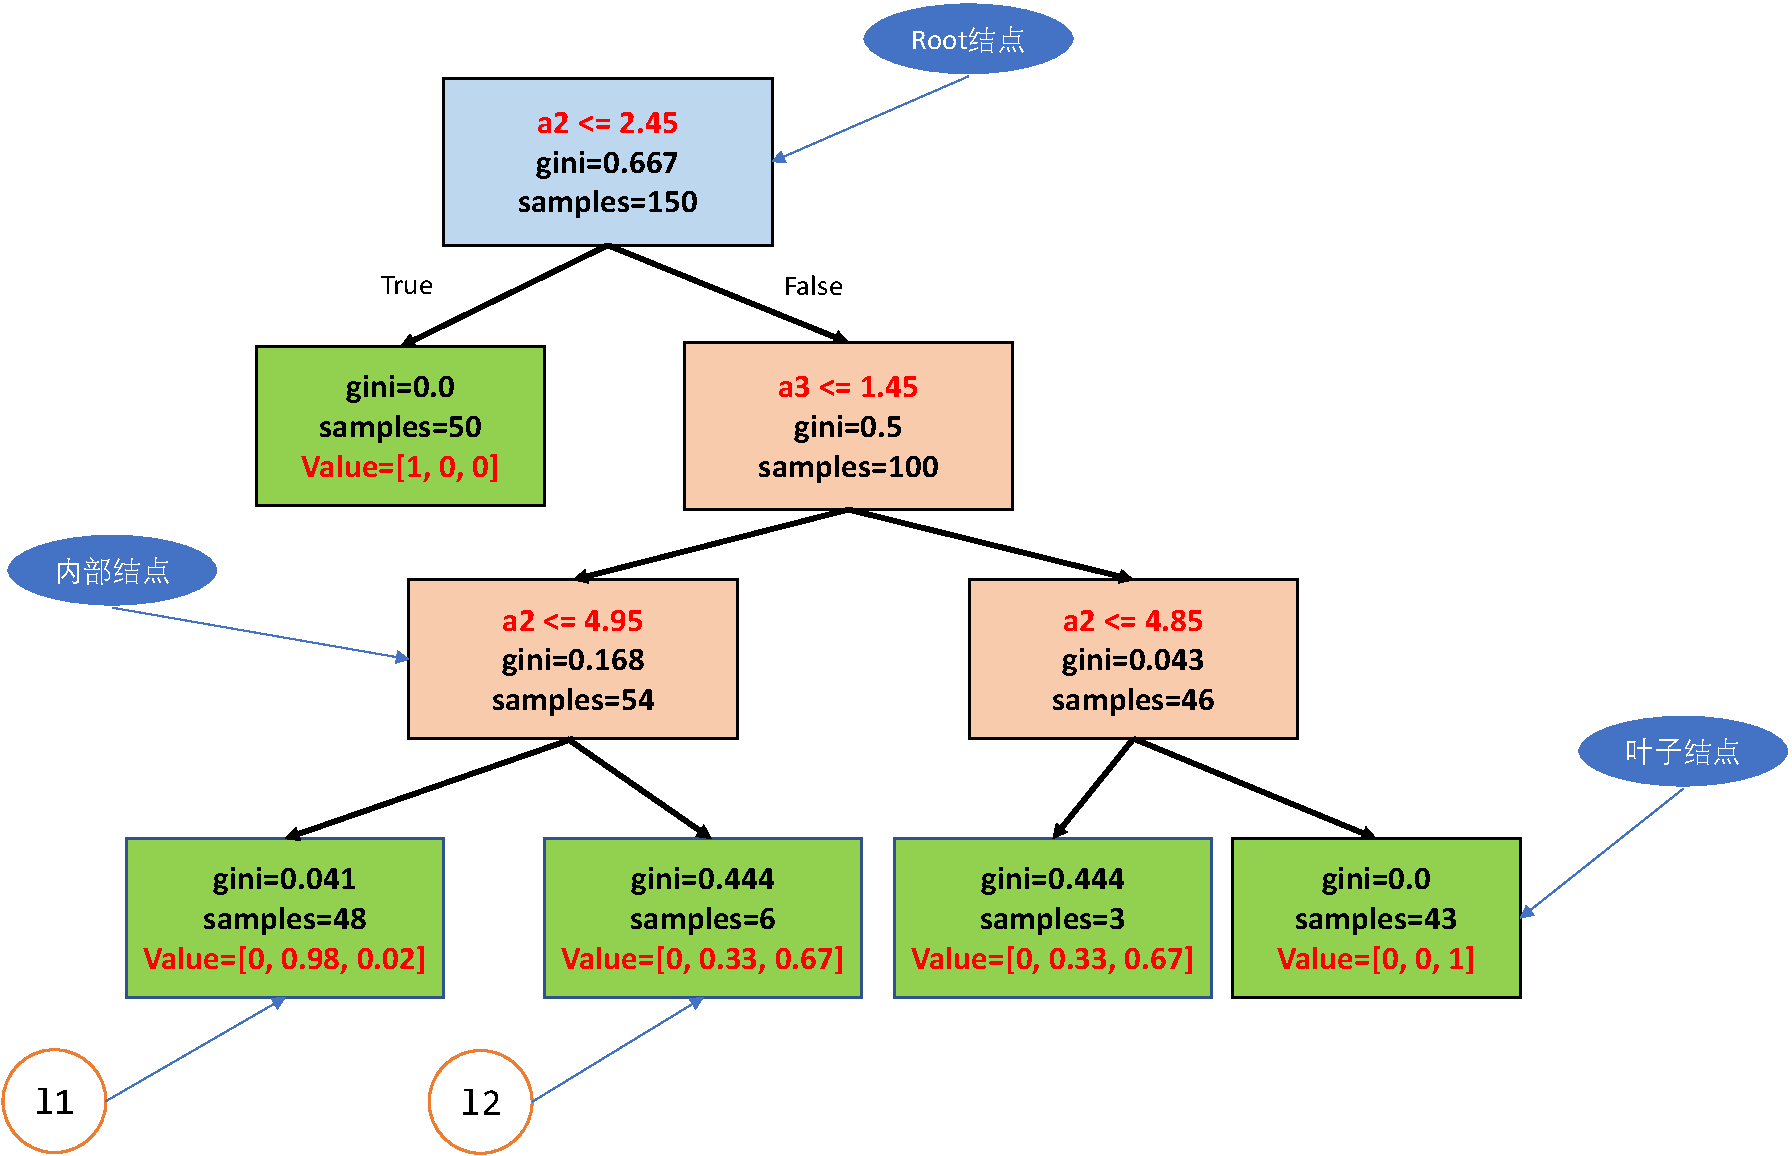
\includegraphics[scale=0.5]{fig2/C3/FLJCS.pdf}%分类决策树
	\caption{分类树}
	\label{fig:分类树结构图}	
\end{figure}

\begin{ex}[分类决策树的SMT公式]\label{分类决策树例子}
图\ref{fig:分类树结构图}为用于莺尾花分类任务的决策树,其中叶子结点$l_1$的路径公式$w_{l_{1}} = (a_2 \le 2.45) \wedge (a_3 \le 1.45) \wedge (a_2 \le 4.95) \wedge (o = v_{l_{1}})$, 其中 $o$为一个约束变量的集合且$o=\{ o_0=p_0, o_1=p_1,o_2=p_2\}$, $v_{l_{1}}$为预测类别的概率集合且$v_{l_{1}}=\{p_0=0,p_1=0.98,p_2=0.02\}$,其中叶子结点$l_2$的路径公式$w_{l_{2}} = (a_2 \le 2.45) \wedge (a_3 > 1.45) \wedge (a_2 > 4.95) \wedge (o = v_{l_{2}})$, 且$o=\{ o_0=p_0, o_1=p_1,o_2=p_2\}$, $v_{l_{2}}=\{p_0=0,p_1=0.33,p_2=0.67\}$。相应的该分类树的 SMT 公式为:$w_{l_{1}} \vee w_{l_{2}} \vee ... \vee w_{l_{j}}$。
\end{ex}

\begin{figure}[!hbt]
\centering
	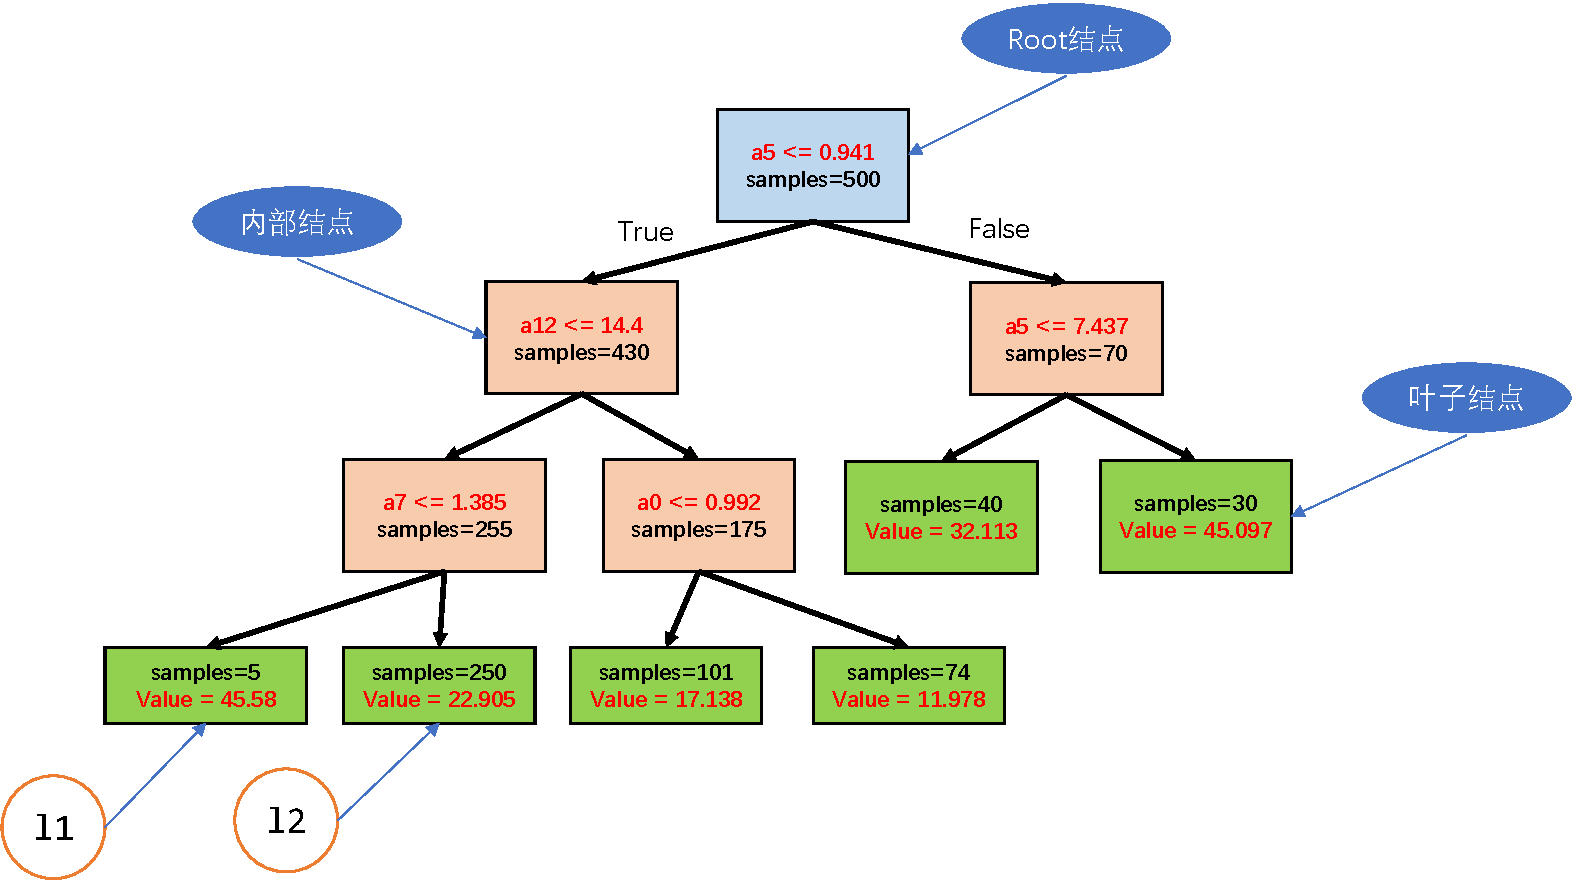
\includegraphics[scale=0.5]{fig2/C3/HGJCS.pdf}%回归决策树
	\caption{回归树}
	\label{fig:回归树结构图}	
\end{figure}


\begin{ex}[回归决策树的SMT公式]\label{回归决策树例子}
图\ref{fig:回归树结构图}为用于预测波士顿房价任务的回归决策树,其中叶子结点$l_1$的路径公式$w_{l_{1}} = (a_5 \le 0.941) \wedge (a_{12} \le 14.4) \wedge (a_7 \le 1.385) \wedge (o = v_{l_{1}})$, 其中 $o$为一个约束变量且$o=v_{l_{1}}$, $v_{l_{1}}$为预测的房价回归值且$v_{l_{1}}=45.58$,叶子结点$l_2$的路径公式$w_{l_{2}} = (a_5 \le 0.941) \wedge (a_{12} \le 14.4) \wedge (a_7 > 1.385 \wedge (o = v_{l_{2}})$, $o=v_{l_{2}}$且$v_{l_{2}}=22.905$。相应的该回归树的 SMT 公式为:$w_{l_{1}} \vee w_{l_{2}} \vee ... \vee w_{l_{j}}$。
\end{ex}

\subsection{随机森林模型的SMT编码}
根据在第二章节关于随机森林基础知识的介绍,我们已经知道它是决策树的组合,之后通过投票机制来得出最终的预测结果。在本节中我们会详细描述如何将随机森林模型编码为 SMT 公式。

(1) 随机森林分类模型编码

随机森林分类模型 $RFC$ 是 $k$ 棵分类树的集合,即 $RFC=\left\langle T_{1}, \ldots T_{k}\right\rangle$。对于一个输入样本$x$来说,其预测类别为在模型$RFC$中所有决策树给出的投票结果。在本文中,我们考虑的软投票的情况。因为有研究表明,基于类概率的投票往往性能会更好。
我们知道每棵分类树的输出都是一组对应于每个类的概率,然后分类模型 $RFC$会将在所有分类树中概率估计平均值最高的预测类别作为预测结果输出。此过程可表示为如下公式:
\begin{equation}\label{eq:1}
RFC(x)=\operatorname{argmax}_{j} \frac{1}{k} \sum_{i=1}^{k} t_{i}^{j}(x)
\end{equation}
其中$t_i(x)$ 表示分类树$T_i$对 $x$的预测类别,$t_{i}^{j}(x)$表示树 $T_i$对类别 $j$ 的预测概率,且 $\sum_{i=1}^{m} t_{i}^{j}(x)=1$, $m$ 表示预测类别的个数。根据随机森林的定义,随机森林的编码是其集合中所有分类树的SMT公式的合取公式。即:
\begin{equation}\label{eq:2}
 RFC: \bigwedge_{i=1}^{k} \Pi\left(T_{i}\right) \wedge\left(\text {out}=\operatorname{argmax} \frac{1}{k} \sum_{i=1}^{k} o_{i}^{j}\right)
\end{equation}
其中变量$o_i$用来约束树$Ti$的输出$t_i(x)$,相应的 $o_{i}^{j}$用来约束预测类别 $j$ 的概率$t_{i}^{j}(x)$, $out$为模型 $RFC$ 的输出约束变量。

(2) 随机森林回归模型编码

随机森林回归模型 $RFR$ 是 $k$ 棵回归树的集合,即 $RFR=\left\langle T_{1}, \ldots T_{k}\right\rangle$。对于一个输入样本$x$来说,其预测结果为在模型 $RFR$ 中所有回归树给出的平均值。我们知道每棵回归树的输出都是一个预测回归值,回归模型 $RFR$ 会将在所有分类树中预测结果的平均值作为预测结果输出。此过程可表示为如下公式:

\begin{equation}\label{eq:3}
RFR(x)=\frac{1}{k} \sum_{i=1}^{k} t_{i}(x)
\end{equation}

其中$t_i(x)$ 表示分类树$T_i$对 $x$的预测值。随机森林的编码是其集合中所有分类树的SMT的合取公式。即:

\begin{equation}\label{eq:4}
RFR:\bigwedge_{i=1}^{k} \Pi\left(T_{i}\right) \wedge\left(\text {out}= \frac{1}{k} \sum_{i=1}^{k} o_{i}\right)
\end{equation}

其中变量$o_i$用来约束树$T_i$的输出$t_i(x)$ ,$out$为模型 $RFR$ 的输出约束变量。

\subsection{GBDT 的 SMT 编码}
GBDT模型的 SMT 公式的编码过程与随机森林模型类似。但对于回归任务和分类任务来说,GBDT 都是以回归树作为基学习器去完成预测任务,所以最终构建的 SMT 公式也会有所区别。

(1) GBDT分类模型的SMT编码

对于分类任务来说,GBDT 模型与随机森林模型不同,GBDT是基于回归树去完成分类预测。对于每个预测类别都会训练对应数目的回归树。例如:GBDT 模型用于一个三分类的任务,指定其基学习器的数目为5,则每个类别都需要训练 5 棵树,总计需要训练15 棵树来完成预测任务。具体来说,GBDT 分类模型GBC是由多个回归树组成的集合,即 $GRC = \left\langle R_{1}, \ldots, R_{c}\right\rangle$ 且 $R_{j}=\left\langle T_{1}^{j}, \ldots, T_{r}^{j}\right\rangle$ , 其中$c$表示的是预测类别的个数, $r$表示回归树的棵树,$R_j$表示类别 j的回归树集合。对于一个输入样本$x$来说,分类模型 $GBC$的预测结果为概率最大的类别,即$GBC(x)=\arg \max _{j}\left(R_{j}(x)\right)$。 则该 SMT 公式可定义为:
\begin{equation}\label{eq:5}
GBC:\bigvee_{j=1}^{c}\left(\arg =j \leftrightarrow \bigwedge_{k=1}^{c} \text {out}_{j}>\text {out}_{k}\right)
\end{equation}

其中变量$o_i$用来约束树$Ti$的输出$t_i(x)$, $out$为模型 $GRC$ 的输出约束变量。

(2) GBDT回归模型的SMT编码

GBDT 的回归模型 $GBR$ 是由多个回归树组成的集合,即 $GBR=\left\langle T_{1}, \ldots, T_{r}\right\rangle$。 对于一个输入样本$x$来说,回归模型 $GBR$ 的预测结果为集合中回归树预测值的总和,即 $GBR(x)=\sum_{i=1}^{r}T_i(x)$。则该 SMT 公式可定义为:
\begin{equation}\label{eq:6}
GBR:\left(\bigwedge_{i=1}^{r} \Pi\left(T_{i}\right)\right) \wedge \left(out=\sum_{i=1}^{r} o_{i}\right)
\end{equation}

其中变量$o_i$用来约束树$Ti$的输出$t_i(x)$, $out$为模型 $GBR$ 的输出约束变量。
\subsection{模型鲁棒性SMT编码}
在之前的小节中,我们已将树模型编码为SMT公式,接下来,我们会基于测试样本去构造该模型鲁棒性的布尔公式。

(1) 单样本的鲁棒性的编码

\begin{define}[特征扰动约束公式]\label{特征扰动约束公式}
若输入样本$x = <a_1,...,a_d>$, 最大扰动为$\epsilon$, 若其对应的对抗性样本为$x'$, 则扰动约束公式为$\Delta(x,x',\epsilon)$:
\begin{equation}\label{eq:7}
\Delta(x, x', \epsilon):\bigwedge_{i=1}^d |a_i-a_i'|\le \epsilon \;\;\;\; (a_i \in x,a_i' \in x')
\end{equation}
\end{define}
\begin{define}[回归模型单样本鲁棒性公式]\label{回归模型单样本鲁棒性公式}
根据定义\ref{回单样本鲁棒性}, 若模型$R$为回归模型, 输入样本$x = <a_1,...,a_d>$,最大扰动为$\epsilon$,对抗性样本为$x'$,则回归模型的单样本鲁棒性公式$\Phi_R$可定义为:
\begin{equation}\label{eq:9}
\Phi_R: R\left(x^{\prime}\right) \wedge \Delta\left(x, x^{\prime}, \epsilon\right) \wedge(|R(x)-out| \ge \delta)
\end{equation}
\end{define}
在公式(\ref{eq:9})中的,回归模型$R$代表在随机森林的分类模型RFR的 GBDT 的回归模型GBR。 至此,我们可以将回归模型的鲁棒性验证问题转换为查找是否存在使得公式$\Phi_R$的可满足的赋值$x'$的问题。如果该赋值$x'$存在,则说明该模型在样本$x$受到扰动的情况下(对抗性样本为$x'$),会预测错误,即不满足鲁棒性;相反,如果赋值$x'$不存在,则说明该模型满足鲁棒性。我们将在下边给出形式化证明。
\begin{define}[分类模型单样本鲁棒性公式]\label{分类模型单样本鲁棒性公式}
根据定义\ref{分单样本鲁棒性}, 若模型$C$为分类模型, 输入样本$x = <a_1,...,a_d>$, 最大扰动为$\epsilon$, 对抗性样本为$x'$, 则分类模型的单样本鲁棒性公式$\Phi_C$可定义为:
\begin{equation}\label{eq:8}
\Phi_C: C\left(x^{\prime}\right) \wedge \Delta\left(x, x^{\prime}, \epsilon\right) \wedge(\text {out} \neq C(x))
\end{equation}
\end{define}
在公式(\ref{eq:8})中的,分类模型$C$代表在随机森林的分类模型RFC的 GBDT 的分类模型GBC。同样的,我们可以将分类模型的鲁棒性验证问题转换为查找是否存在使得公式$\Phi_C$的可满足的赋值$x'$的问题。如果该赋值$x'$存在,该分类模型$C$不满足鲁棒性;相反,如果赋值$x'$不存在,则说明该模型满足鲁棒性。

\begin{theorem}\label{th:7}
给定一个模型$C=<T_1,...,T_k>$,输入样本$x\in X^d$,其对应的鲁棒性公式为$\Phi_C$。 如果$\Phi_C$是可满足的,则其真赋值$x' \in X^d$是该模型的对抗性样本,该模型$C$不满足鲁棒性;反之,如果$\Phi_C$不满足的,则模型$\Phi_C$相对于$x$满足鲁棒性。
\end{theorem}

\begin{proof}
我们以随机森林分类模型为例,给出如下的证明。

假设$\Phi_C$是可满足的,则存在真赋值$x'$,并且 $O=\{o_i|1\le i \le k\}$。根据公式(\ref{eq:2})和公式(\ref{eq:7}),我们可以得出:$(out \ne RFC(x))$成立,并且在模型RFC 中的每个决策树公式$\Pi(T_i)$
都成立。在不失一般性的前提下,让我们考虑树$T_1$的公式$\Pi(T_i)$为True的情况,则必然存在一个真赋值 $o_1 \subset O$。我们首先需要证明树$T_1$对于$x'$的预测结果就是真赋值$o_1$ ,即 $t_1(x') = o_1$。根据公式(\ref{eq:10}),我们可以得出至少有一个叶子路径公式的赋值为True。参考决策树的定义,除了根结点$n_0$之外,每个内部结点只有一个前驱结点,因此我们可以确保只有一个叶子路径公式的赋值为True。假设叶子公式为$w(l_0)$,叶子$l_0$的值为$v_{l_0}$。然后,考虑在树$T_1$预测输入样本$x'$的决策过程。当$x'$到达内部结点$n$时,如果特征 $a'\in x'$满足特征阈值公式$(s_n=(a' \le \eta))\in w(l_0)$,则$x'$将被传递到给左孩子结点,如果不满足$s_n$的话,将会被传到右孩子结点。从根结点递归应用该决策规则,最终$x'$将会落到在叶子$l_0$,最终的预测结果就是该叶子的值,即$t_1(x')=v_{l_0}$。根据公式(\ref{eq:2}),则$o_1 = v_{l_0}$,那么我们可以得出$t_1(x') = o_1$的结论。类似地,我们可以得出$t_2(x') = o_1,...,t_k(x')=o_k$。

为了便于描述,我们可以将公式(\ref{eq:1})简化为$RFC(x')=argmax(T(x'))$。通过公式(\ref{eq:2}),我们得出$out=argmax(O)$,则$RFC(x')=out$。我们已经知道$(out \ne RFC(x))$为True,因此赋值$x'$是模型$RFC$的对抗性样本。类似地,如果$\Phi_C$不满足的话,则表明不存在这样的对抗性样本$x'$,即该模型相对于$x$满足鲁棒性。即证。
\end{proof}

(2) 全局鲁棒性的编码

\begin{define}[回归模型全局鲁棒性公式]\label{回归模型全局鲁棒性公式}
根据定义\ref{回全局鲁棒性}, 设$R$为回归模型,$N$为测试样本集合。如果$N$至少存在$\rho \cdot |N|$个样本,使得$R$满足回归模型单样本鲁棒性,则$R$满足回归模型的全局鲁棒性。则回归模型的全局鲁棒性公式$\Phi_{GR}$可定义为:
\begin{equation}\label{eq:11}
\bigwedge_{i=1}^{|N|}\left(\Phi_{i} \Leftrightarrow q_{i}\right) \wedge \sum_{i=1}^{|N|} q_{i} \geq \rho \cdot|N|
\end{equation}
\end{define}
在公式(\ref{eq:11})中的,回归模型$R$代表在随机森林的分类模型RFR的GBDT的回归模型GBR。

\begin{define}[分类模型全局鲁棒性公式]\label{分类模型全局鲁棒性公式}
根据定义\ref{分全局鲁棒性}, 设$C$为分类模型,$N$为测试样本集合。如果$N$至少存在$\rho \cdot |N|$个样本,使得$C$满足分类模型的单样本鲁棒性,则$C$满足分类模型的全局鲁棒性。则分类模型的全局鲁棒性公式$\Phi_{GC}$可定义为:
\begin{equation}\label{eq:12}
\bigwedge_{i=1}^{|N|}\left(\Phi_{i} \Leftrightarrow q_{i}\right) \wedge \sum_{i=1}^{|N|} q_{i} \geq \rho \cdot|N|
\end{equation}
\end{define}
在公式(\ref{eq:12})中的,分类模型$C$代表在随机森林的分类模型RFC的GBDT 的分类模型GBC。

\section{SMT 求解器}
 随着对于SMT研究和技术的进步,现在已经有了一些功能强大和复杂的SMT求解器,例如Alt-Ergo \cite{bobot2008implementing}、 Beaver \cite{jha2009beaver},Boolector\cite{brummayer2009boolector}、MathSAT5\cite{cimatti2013mathsat5}、 openSMT\cite{bruttomesso2010opensmt}、 SMTInterpol\cite{christ2012smtinterpol}、SONOLAR\cite{peleska2011automated}、STP\cite{ganesh2007decision}、veriT\cite{bouton2009verit}、Yices\cite{dutertre2006yices}、Z3\cite{de2008z3}等可以快速扩展的应用程序集。目前的应用领域包括处理器验证,等价性检查,有界和无界模型检查,谓词抽象,静态分析,自动测试用例生成,类型检查、计划、调度和优化等。在很多神经网络的验证工具\cite{sato2019formal,2017Safety,2019Synthesizing,2017Formal}中,选择Z3求解器作为其底层的求解器。在本文的鲁棒性验证框架中,我们同样将Z3求解器作为SMT求解器,但需要注意的是,框架也支持其他主流的 SMT求解器。

Z3有着高效而且全面的的求解能力,它是开源的,并且支持当前所有的SMT理论,并且提供了多种 API 接口。在本框架中,因为我们框架的实现是基于 Python 语言的,所以调用其Python API。我们会将 SMT 编码模块生成的公式转化为Z3求解器可接受的公式形式,之后利用Z3求解器去对该公式进行求解。

根据对SMT公式的求解结果,Z3会返回“UNSAT”和“SAT”两种结果。“UNSAT”表示无法找到该公式的可行解,根据我们给出的模型鲁棒性的定义,此结果表示该模型满足鲁棒性。 “SAT”结果存在该公式的可行解,则表明该模型不满足鲁棒性,返回的可行解即为该模型的一个对抗性样本。

\section{验证结果分析模块}
 验证结果分析模块的基本功能是统计和分析验证结果,如待验证树模型的鲁棒性值,满足鲁棒性的样本个数和所占的百分比,验证失败或验证超时的样本个数或所占的百分比等。除此之外,在下一章节关于树模型可解释研究中提出的算法也在该模块实现。
\section{对抗性样本生成模块}
对抗性样本生成模块是为了生成树模型对抗性样本。当模型的鲁棒性验证结果为不满足的情况时(即求解器返回的结果为 “SAT”),此时求解器还会返回一个可行解 $x'$,$x'$为该模型的一个对抗性样本。但$x'$并不能直接作为对抗性样本输入到模型中,必须要按照原始样本的数据格式进行二次处理才能成为模型可接受的输入形式。该模块提供了将求解器生成的反例转换为树模型可接受的输入样本格式即对抗性样本的功能。
\section{本章小结}
在本章节中,我们介绍了树模型鲁棒性验证框架的设计与实现部分。我们详细描述了该框架的各个模块的设计和实现的细节,包括了树模型解析模块,样本预处理模块,SMT 编码模块等。我们的核心工作是对树模型及其鲁棒性的 SMT公式编码的设计,展示了从决策树到整体树模型的编码过程,对底层所用的 Z3 求解器也做了介绍。